%%%%%%%%%%%%%%%%%%%%%%%%%%%%%%%%%%%%%%%%%%%%%%%%%%%%%%%%%%%%%%%%%%%%%%%%%%%%%%%%%%%%
% Do not alter this block (unless you're familiar with LaTeX
\documentclass{article}
\usepackage[margin=1in]{geometry} 
\usepackage{amsmath, amsthm, amssymb,amsfonts, fancyhdr, color, comment, graphicx, environ}
\usepackage{xcolor}
\usepackage{mdframed}
\usepackage[shortlabels]{enumitem}
\usepackage{indentfirst}
\usepackage{hyperref}
\usepackage{algorithm2e}
\usepackage{graphicx}
\usepackage{wrapfig}
\usepackage{hyperref}
\usepackage{listings}
\lstset{ 
  language=R,                     % the language of the code
  basicstyle=\normalsize\ttfamily, % the size of the fonts that are used for the code
  numbers=left,                   % where to put the line-numbers
  numberstyle=\normalsize\color{gray},  % the style that is used for the line-numbers
  stepnumber=1,                   % the step between two line-numbers. If it is 1, each line
                                  % will be numbered
  numbersep=5pt,                  % how far the line-numbers are from the code
  backgroundcolor=\color{white},  % choose the background color. You must add \usepackage{color}
  showspaces=false,               % show spaces adding particular underscores
  showstringspaces=false,         % underline spaces within strings
  showtabs=false,                 % show tabs within strings adding particular underscores
  frame=single,                   % adds a frame around the code
  rulecolor=\color{black},        % if not set, the frame-color may be changed on line-breaks within not-black text (e.g. commens (green here))
  tabsize=2,                      % sets default tabsize to 2 spaces
  captionpos=b,                   % sets the caption-position to bottom
  breaklines=true,                % sets automatic line breaking
  breakatwhitespace=false,        % sets if automatic breaks should only happen at whitespace
  keywordstyle=\color{black},      % keyword style
  commentstyle=\color{gray},   % comment style
  stringstyle=\color{teal}      % string literal style
} 
\hypersetup{
    colorlinks=true,
    linkcolor=blue,
    filecolor=magenta,      
    urlcolor=blue,
}


\pagestyle{fancy}


\newenvironment{problem}[2][]
    { \begin{mdframed}[backgroundcolor=gray!20] \textbf{#1 #2} \\}
    {  \end{mdframed}}

% Define solution environment
\newenvironment{solution}
    {}

\renewcommand{\qed}{\quad\qedsymbol}

% prevent line break in inline mode
\binoppenalty=\maxdimen
\relpenalty=\maxdimen

%%%%%%%%%%%%%%%%%%%%%%%%%%%%%%%%%%%%%%%%%%%%%
%Fill in the appropriate information below
\lhead{Pengju Zhang}
\rhead{CSC-424} 
\chead{\textbf{Individual Report}}
%%%%%%%%%%%%%%%%%%%%%%%%%%%%%%%%%%%%%%%%%%%%%

\begin{document}
%problem 1
\begin{problem}{}
In this final individual milestone, you will submit a starting draft of your final project individual report.  See the final project instructions for details and look closely at the rubric.  You should describe what you have been working on here at the beginning and where you are thinking to take your analyses in the final weeks of the course.  Note that this is not a zero-sum game.  You may report on material that you have collaborated on with your partners, and it does not have to be solely your work, but you should be able to describe in detail how you contributed.
\end{problem}
\begin{solution}
\href{run:./src/clustering.r}{ (Clustering Analysis Source Code)}
\newline
My part is focusing on cleaning data and clustering analysis.
	\begin{figure}[h]
		\centering
		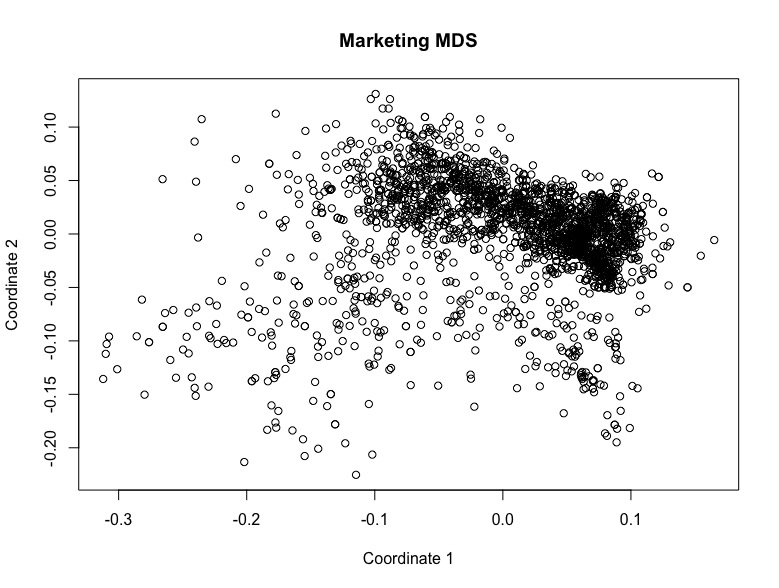
\includegraphics[width=0.7\textwidth]{General MDS.jpeg}
		\caption{General MDS Plot}
	\end{figure}
\newline
	Initial we want to find the pattern through general MDS plot, but there is not clue to demonstrate a clear cluster in my graph. Then I try to displays a measure of how close each point in one cluster is to points in the neighboring clusters and thus provides a way to assess parameters like number of clusters visually through silhouette plot, but the silhousette width with less than 0.25 indicate the very little substantial  structure has been found. If we try to visualize the clusters from 2 to 8, clearly our clustering plot shows a lot of random pattern and most of them are cross with each other.
\newline
	Finally, I use elbow method and cluster dendrogram to find the number of optimal clusters are 2 and 3, and they both show very clear clusters in our graphs. In order to find the which variables can be potentially described by 2 or 3 classes, I use histogram to go through all variables, Income in this case is equally separated into two parts, so I use mean value as critical point and label then as "Lower" and "Higher" according to their value compare to its mean. Then I re-plot it again, it shows me the clustering plot has very high correlation with Income, “Higher” are most on the left, “Lower” on right (Figure 9).
	\begin{figure}[h]
		\centering
		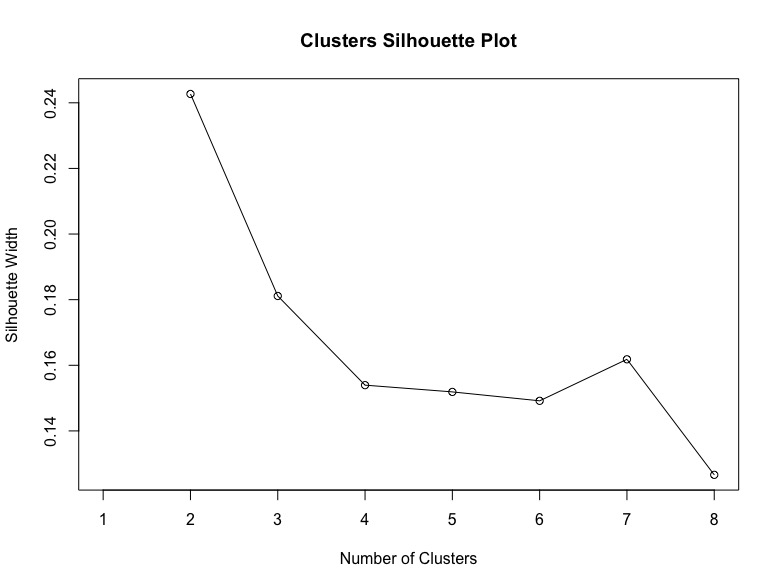
\includegraphics[width=0.7\textwidth]{Silhouette Plot.jpeg}
		\caption{Silhouette Plot}
	\end{figure}
	\begin{figure}[h]
		\centering
		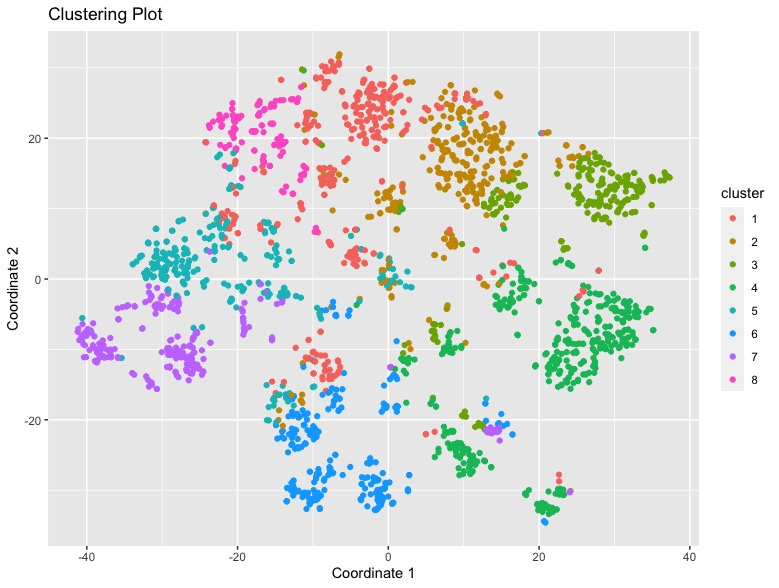
\includegraphics[width=0.7\textwidth]{Clustering Plot.jpeg}
		\caption{Clustering Plot}
	\end{figure}
	\begin{figure}[h]
		\centering
		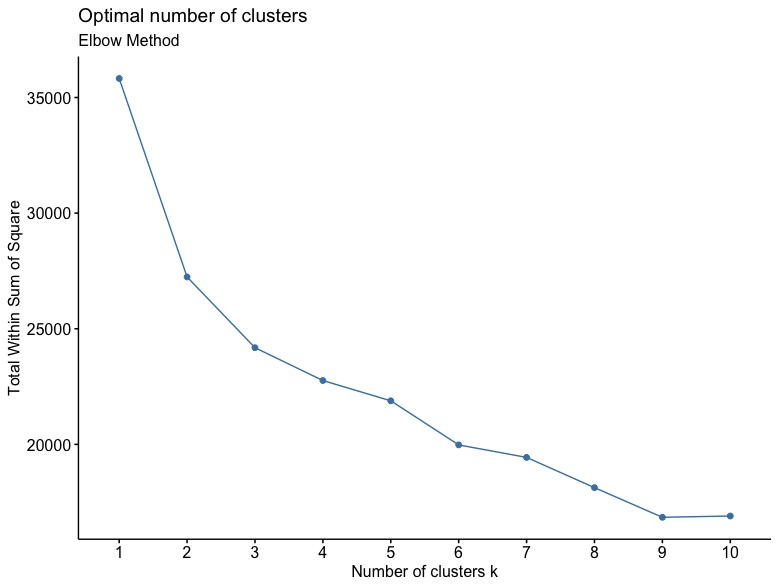
\includegraphics[width=0.7\textwidth]{Elbow Method.jpeg}
		\caption{Elbow Method Plot}
	\end{figure}
	\begin{figure}[h]
		\centering
		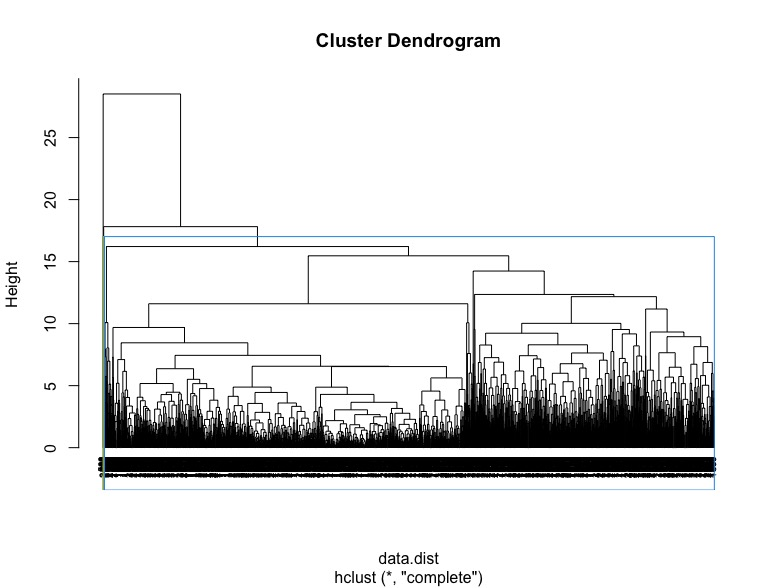
\includegraphics[width=0.7\textwidth]{Cluster Dendrogram.jpeg}
		\caption{Cluster Dendrogramt}
	\end{figure}
	\begin{figure}[h]
		\centering
		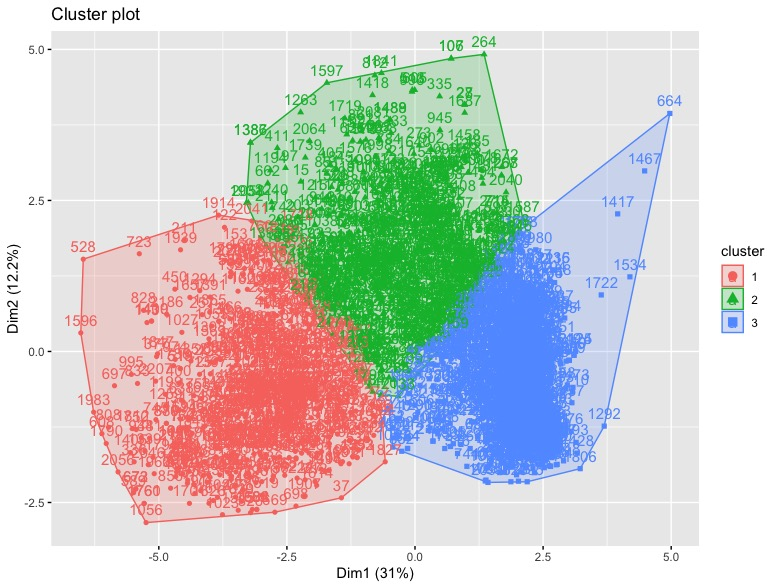
\includegraphics[width=0.7\textwidth]{Cluster Plot (Reduced).jpeg}
		\caption{Cluster Plot with 3 clusters}
	\end{figure}
	\begin{figure}[h]
		\centering
		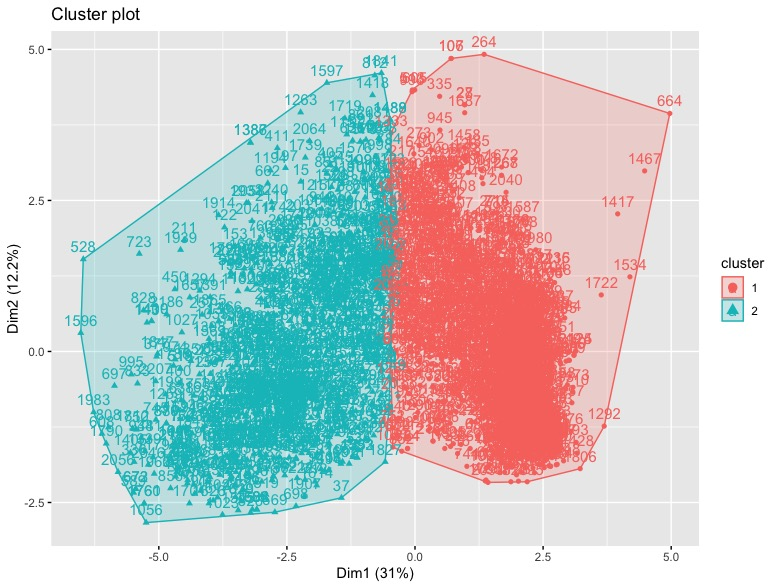
\includegraphics[width=0.7\textwidth]{Cluster Plot Two.jpeg}
		\caption{Cluster Plot with 2 clusterst}
	\end{figure}
	\begin{figure}[h]
		\centering
		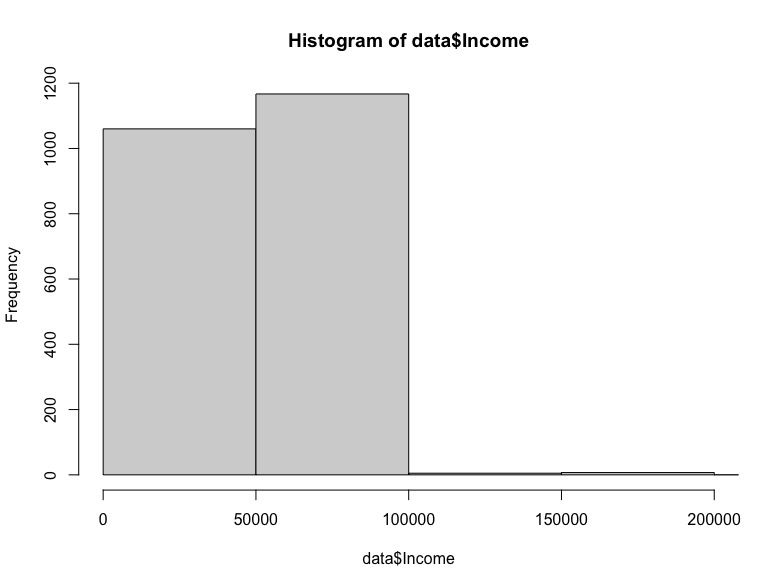
\includegraphics[width=0.7\textwidth]{Histogram.jpeg}
		\caption{Income Histogram}
	\end{figure}
	\begin{figure}[h]
		\centering
		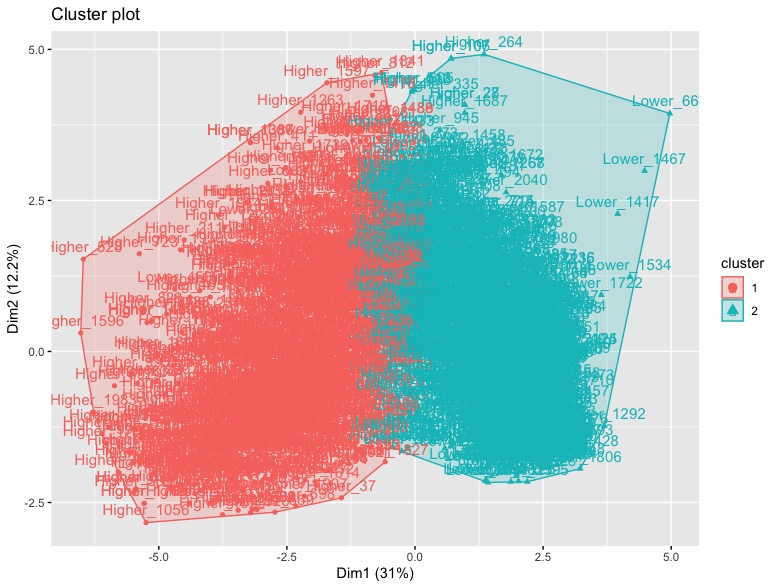
\includegraphics[width=0.7\textwidth]{Result Clustering.jpeg}
		\caption{Final Clustering}
	\end{figure}
\end{solution}

\end{document}